\chapter{A sketch of lattice field theory}\label{ch:LFT}

LFT was first dreamt up by Kenneth Wilson\footnote{Wilson was more of a condensed
matter theorist at that time. Back then, people were still working out the SM,
fueled by a cavalcade of rapid experimental discoveries of new particles. For
Wilson, particle physics seemed very exciting, and he wanted in on the action.
Since his expertise was not in high energy theory, he took an approach more
informed by condensed matter, which led to his lattice formulation. Indeed, his
approach makes plain many powerful, formal correspondences between lattice field
theories and {\it spin models}\index{spin model}, which are models that explain
how magnets work by imagining them as a solid block of interacting spins.} 
in 1974~\cite{wilson_confinement_1974}.
He used this formalism to explain a phenomenon called {\it quark
confinement}\index{quark confinement}, which is the observation that one never
finds a quark alone in nature. He considered an infinitely heavy quark-antiquark
pair and calculated its potential energy in the lattice formalism. He found
\begin{equation}
V_{\bar{q}q}(r)\sim\frac{A}{r}+\sigma r,
\end{equation}
where $r$ is the separation between the quarks and $\sigma$ is a positive 
constant called the {\it string tension}\index{string tension}. The first term 
is reminiscent of the Coulomb potential energy from electrodynamics, so it is 
often called the ``Coulomb part". In contrast with the EM Coulomb interaction, 
this part of the potential, is repulsive between the quark-antiquark pair.
When $r$ is small, this term dominates. When $r$ is large, the second term
dominates, and the potential increases with $r$.
How this leads to confinement is sketched pictorially
in \figref{fig:confinement}. 

\begin{figure}
  \centering
  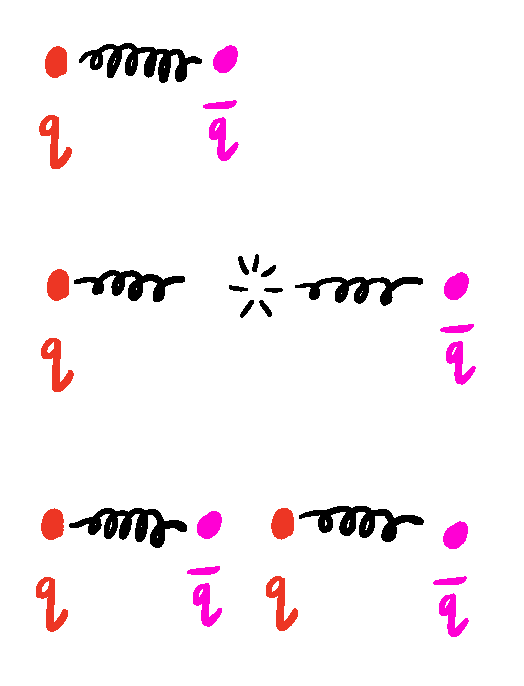
\includegraphics[width=0.8\linewidth]{figs/confinement.pdf}
  \caption{A sketch of the confinement phenomenon. {\it Top}: A quark-antiquark
pair bound together through the strong interaction. {\it Middle}: The quark and
antiquark are separated, which increases the potential energy between the
quarks. Eventually this energy becomes so high, the binding ``breaks".
{\it Bottom}: The binding breaks because the potential energy exceeds the rest
mass energy of another quark-antiquark pair. Therefore it is energetically
favorable to generate such a pair from the vacuum, which is what is shown here.
Thus from one quark-antiquark pair there spawns two.} 
  \label{fig:confinement} 
\end{figure}

At first, people thought that lattice simulations would not be computationally
viable, Wilson included. This attitude changed in 1979 when Michael Creutz, 
working at Brookhaven
National Lab, carried out the first lattice study, at that time using the gauge
group\footnote{You can think of this group like a simplified version of
$\SU(3)$, which again is the gauge group corresponding to real-world gluons.
$\SU(2)$ has a lot of qualitative similarities to $\SU(3)$, while being
computationally much, much cheaper. Therefore lattice practitioners sometimes
like to use $\SU(2)$ as a testing ground. In fact when I was a grad student, the
systems I studied only had $\SU(2)$ ``gluons".} $\SU(2)$~\cite{creutz_monte_1980}. 
Creutz's success excited the high
energy community very much. Early computers were far too weak to simulate realistic
quarks, so studies were limited to theories with gluons only. Over the last
decades, advancements in computer hardware and computing algorithms, along with 
better theoretical control over implementations of lattice field theories on
computers, have allowed us to simulate most of the QCD sector. State-of-the-art 
calculations include, in addition to gluons, physically realistic up, down,
strange, and charm quarks.

I now attempt to give a sketch of how LFT works. In nature we
exist in a 4-$d$ space-time; correspondingly LFT will have a 4-$d$ domain. The
trick with LFT is to imagine that the space-time is {\it
discrete}\index{discrete}; i.e. that there is a minimum distance between points.
One usually looks at a small region of space-time, represented by a 4-$d$
box\footnote{In higher dimensions, one sometimes calls rectangles
{\it orthotopes}\index{orthotope}.}. Setting up this discrete lattice renders
the previously uncountably infinite domain finite and countable. Since the
theory can now be specified by finitely many numbers, we are able to store it in
a computer's memory.

At this stage I would like to emphasize that {\it the lattice is in no way
real}. It is a calculational crutch that allows us to utilize methods of scientific
computing\footnote{There are other technical advantages as well, but getting
into them is far beyond the scope of these notes.}. As we increase the finite
number of discrete points on our lattice while simultaneously decreasing the
lattice spacing, we obtain an increasingly accurate depiction of reality in that
space-time box. By extrapolating to the limit of zero lattice spacing, we hope
to lose all reference to the lattice; put another way, our crutch disappears.

In the following sections, I will try to explain these ideas in a little more
detail. I don't expect you to understand things fully, because I am not
explaining them fully. It is enough for you to have a heuristic understanding of
what a lattice calculation entails. 


\section{Defining the lattice}

Let $N_{1},N_{2},N_{3},N_{4}\in \N\cup\{0\}$. The {\it lattice} ${\Lambda}$ is defined by
\begin{equation}
  {\Lambda}\equiv\{\fvec{x}\suchthat x_\mu=a\,n_\mu,\,n_\mu< N_\mu,\,
      \mu=1,2,3,4\}.
\end{equation}
Here $a$ is called the \index{lattice spacing}{\it lattice spacing}.
The subscript $\mu$ indicates the $\mu$-component of the four vector $\fvec{x}$.
We identify $N_1$, $N_2$, and $N_3$
as the extensions of the lattice in the spatial directions,
and $N_4$ is taken to be the extension in the time
direction. Matter fields 
are defined on the \index{site} {\it sites} $\fvec{x}\in\Lambda$. We shall
take the lattice to have periodic\footnote{Real life does not have periodic BCs.
We like to implement periodic BCs on the lattice in part because they allow for
symmetries under translations. You may protest that because real life doesn't
have periodic BCs, it is not reasonable to implement them on the lattice. One
reason this can be justified is as follows: Physical quantities that are small
compared to the box size tend not to ``feel" the BCs very strongly. This
manifests in principle as a systematic error that decreases, often
exponentially, with increasing box size. As long as the box is large enough, 
this systematic error is swallowed by
the statistical error, i.e. it is negligible.} boundary conditions (BCs), i.e.
\begin{equation}\label{eq:PBC}
  \fvec{x}+aN_{\mu}\hat{\mu}=\fvec{x},
\end{equation}
where $\hat{\mu}$ is the unit vector\footnote{Hence $a\hat{\mu}$ marches one 
step in the $\muh$-direction.} in the direction indicated by $\mu$.
An example of this setup in two dimensions is given in \figref{fig:lattice}.

\begin{figure}
  \centering
  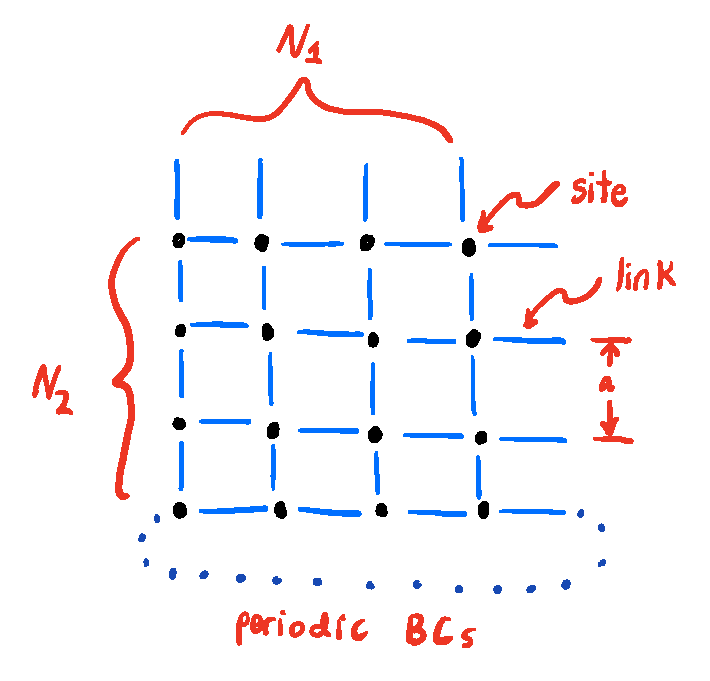
\includegraphics[width=\linewidth]{figs/lattice2d.pdf}
  \caption{A 2-$d$ lattice with $N_1=N_2=4$. Sites are indicated by black dots
and links are indicated by blue lines. Matter fields live on the sites and gauge
fields live on the links connecting the sites. The dotted, dark blue line 
indicates periodic BCs,
i.e. if I start at the bottom-right site and march one step to the right
($\mu=1$ direction in this example), I will end up at the bottom-left site.}
  \label{fig:lattice} 
\end{figure}

Let us explore some of the consequences of treating space-time as discrete
and putting it in a box.
There are many, but we will here focus only on a few of the most easy-to-grasp
ones. First of all, derivatives are given by
by finite differences,
\begin{equation}\label{eq:dertodiff}
  \partial_\mu f(\fvec{x})\to\Delta_{\mu}f(\fvec{x})\equiv\frac{f(\fvec{x}+a\hat{\mu})
                                                   -f(\fvec{x}-a\hat{\mu})}{2a}.
\end{equation}
Note that if one takes the limit $a\to0$, one recovers the definition of a derivative.
We similarly replace integrals with sums,
\begin{equation}\label{eq:inttosum}
  \int \dd[4]{\fvec{x}}f(\fvec{x})\to a^4\sum_\fvec{x}f(\fvec{x}).
\end{equation}
In the limit $a\to0$, letting the number of sites grow to infinity, while
keeping the box size fixed, one gets a Riemann sum, i.e. one gets the familiar
integral again. 
This limiting procedure is called the {\it continuum limit}\index{continuum
limit}, and we expect that we recover real-world results in that limit. 
The continuum limit is shown schematically in \figref{fig:climit}.

\begin{figure}
  \centering
  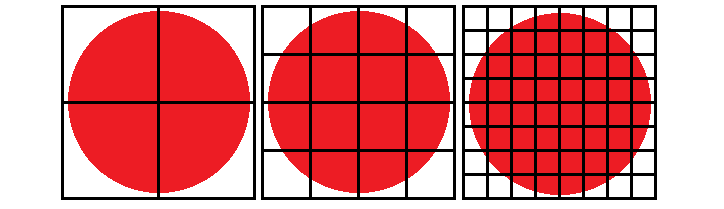
\includegraphics[width=0.9\linewidth]{figs/continuumlimit.png}
  \caption{A schematic representation of the continuum limit. The
           red object represents some physical quantity. As the
           images progress to the right, the lattice spacing decreases
           while the number of sites increases, increasing the resolution.}
  \label{fig:climit}
\end{figure}


There are also some ways physics gets changed when placed on a
discrete lattice in a box, rather than existing in a continuous space-time of
infinite size. In \secref{sec:QM}, we saw that each elementary particle has a
characteristic wavelength. On a finite, discrete lattice, the allowed wavelengths 
of particles are limited.
Heuristically, the lattice does not accommodate particles with a wavelength
smaller than $a$. It also does not accommodate particles whose wavelength is
longer than the box size. This can distort results on a single lattice. The
distortion weakens as one decreases the lattice spacing and increases the box
size, sort of like how a picture gets clearer when one increases the resolution
of a camera. Again, the expectation is that these effects disappear completely
in the continuum limit. 


\section{Constructing measurable quantities}

For the remainder of this chapter, we are going to forget about matter fields.
Again the purpose of these notes is to give the reader an intuitive
understanding of LFT, and introducing fermion fields gives rise to some
technical challenges. Therefore we are going to restrict our attention to a
theory with gauge fields only, i.e. a theory with gluons as the only particles.
Such theories are sometimes called {\it pure gauge} theories\footnote{If the
gauge group is $\SU(3)$ like it is with QCD, we may even call it a pure
$\SU(3)$ theory.}, and we call
pure gauge theories on the lattice {\it lattice gauge theories} (LGT).

Now that we've sacrificed all particles but the gluon, you may worry there is no
physics remaining from which one can learn something. Thankfully it turns out
that a theory with only gluons and a theory with quarks that have infinite mass
are formally equivalent. Thus leaving out quarks that are already heavy to begin
with, such as the charm quark, is often a good approximation. For the lighter
quarks, one generally picks up some non-negligible systematic error that is not 
always easy to predict. 

Next we define the building blocks necessary to construct gluonic observables on the
lattice. The directed {\it link}\index{link}\footnote{In some older texts one
also sometimes sees the phrase ``link variable".\index{link variable}} 
connects $\fvec{x}$ with the
neighboring point $\fvec{x}+a\hat{\mu}$. We indicate it as 
$U_\mu(\fvec{x})\in \SU(3)$. Since we will be interested in $\SU(3)$ for the
remainder of the text, we denote the identity matrix in $\SU(3)$ as $\id$.
A link is
indicated in \figref{fig:lattice}.
We associate to any path $\mathcal{C}$ one can draw on the lattice
the ordered product of its links  $U(\mathcal{C})$.
If we follow a path and then reverse our steps, we should end
up back where we started; hence
\begin{equation}
  U_{-\mu}(\fvec{x}+a\hat{\mu})U_\mu(\fvec{x})=\id.
\end{equation}
Furthermore $U^\dagger(\fvec{x})U(\fvec{x})=\id$, since $\SU(3)$ is a unitary
group, so we can see the effect
of the dagger on links:
\begin{equation}
  U_\mu^\dagger(\fvec{x})=U_{-\mu}(\fvec{x}+a\hat{\mu}).
\end{equation}
Let $\mathcal{C}_{\fvec{x}}$ be a path on the lattice that originates and
terminates at the point $\fvec{x}$. The corresponding {\it Wilson loop} is
defined by \index{Wilson!loop}$\tr U(\mathcal{C}_{\fvec{x}})$.
All of our observables will be Wilson loops of some kind.

The first observable we will look at is the so-called plaquette.
A\index{plaquette}
{\it plaquette} is the
smallest Wilson loop, an oriented square of side length $a$ with
corresponding link product
\begin{equation}
  \plaq_{\mu\nu}(\fvec{x})=U_\mu(\fvec{x})U_\nu(\fvec{x}+a\hat{\mu})
                        U^\dagger_\mu(\fvec{x}+a\hat{\nu})U^\dagger_\nu(\fvec{x}).
\end{equation}
It turns out that the plaquette is related to the gluonic energy density; i.e.
\begin{equation}\label{eq:edensity}
\ev{\tr\plaq_{\mu\nu}(\fvec{x})}\sim \frac{E}{6V_4}\equiv\epsilon,
\end{equation}
where $V_4$ is the number of sites on the 4-$d$ lattice. The factor 6 comes
because every site in 4-$d$ LGT touches six plaquettes\footnote{In $n$
dimensions, each site $\fvec{x}$ has $n!/2(n-2)!$ positively oriented (the links
curve in the CCW direction) plaquettes
with a link starting at $\fvec{x}$ and pointing away from it. This is equal to the
number of unique combinations of directions. Each link has $2(n-1)$ staples
attached to it.}. The lattice representation of a physical observable is called an {\it
interpolator}; hence the plaquette is an interpolator for the energy density.


In \equatref{eq:edensity}, the desired observable we want to learn about the
system is its energy density. In practice, we can estimate the LHS on one
lattice by calculating the average plaquette on that lattice, i.e. we calculate
the plaquette at every site for all six orientations, then take the arithmetic
mean. This gives us a {\it measurement} of the energy density on the $i\nth$
lattice,
\begin{equation}
\epsilon_i=\frac{1}{6V_4}\sum_{\fvec{x},\mu<\nu}\tr\plaq_{\mu\nu}(\fvec{x}).
\end{equation} 
We will discuss how one generates the $i\nth$ lattice in \secref{sec:steps}.



\section{Recovering numbers with units}

Lattice computations deliver quantities
\begin{equation}\label{eq:latticemass}
M=am,
\end{equation} 
where
$m$ is some physical mass. For example $m$ could be the proton mass in [MeV].
The lattice spacing $a$ has units of [MeV$^{-1}$] (equivalently units of
length), which means that $M$ is unitless. We sometimes like to 
think about $a$ being unitless with $a=1$, which we call
{\it lattice units}\index{units!lattice}. This is a useful way to think
when you consider that a lattice is implemented on the computer. For
instance a space-time point on the lattice will be represented as an integer
tuple\footnote{More precisely, space-time will be represented as an array. One
has to find a bijection between space-time points on the lattice and array
indices, which is called {\it indexing}\index{indexing}. The indexer is used all
the time; therefore how one implements an indexer can have a sizable impact on
the performance of the code.} in the computer $(n_1,n_2,n_3,n_4)$, 
which naturally has no units, and it
is furthermore separated by its nearest neighbors by 1.
Moreover, when starting a brand new project, we are often in a situation where
we don't yet know the lattice spacing.

This raises the obvious question of how one determines $a$. One strategy is to
pick a mass that you already know from experiment. The above example of the
proton is well known, i.e. in that case we know $m$. Knowing $m$, one recovers
the lattice spacing as
\begin{equation}
a=\frac{M}{m}.
\end{equation}
Of course, there are many quantities we know experimentally. Depending on the
project, it may be advantageous to use one mass over another. The act of
choosing a mass to use to determine $a$ is called {\it scale
setting}\index{scale setting},  
and commonly one says something like ``we set the scale with the proton mass."
In this example, we call the proton mass the {\it reference
scale}\index{reference scale}.

Once we know $a$, we are able to determine any physical quantity, so long as we
know its interpolator. This is one of the most elegant characteristics of LFT:
It takes only one input parameter, the reference scale, and everything else
with physical units can be calculated from that, using another equation with the
form \eqref{eq:latticemass}.



\section{Computer implementation}

The goal of a lattice program is to estimate the expectation value of some
physical observable $X$, $\ev{X}$, by randomly generating configurations $C$
distributed with probability $e^{-E(C)}\dd C$, where $E(C)$ is the energy of that
configuration. Remember from \secref{sec:QM}, we know that quantum physics tells
us we are limited to knowing expectation values of experimental outcomes rather
than the exact experimental outcome itself.

Extracting this expectation value generally works as follows:
On each configuration $C_i$, we make a measurement $X_i$, which we can think of
as a random variable. The average
\begin{equation}\label{eq:arithmeticaverage}
  \bar{X}=\frac{1}{\nconf}\sum_{i=1}^{\nconf} X_i,
\end{equation}
where $\nconf$ is the number of generated configurations,
serves as the estimator for $\ev{X}$. From the CLT 
we know that, provided we did everything correctly, $\ev{X}$ should
be at most $\sigma_{\bar{X}}$ away from $\bar{X}$ about 68\% of the time.
Provided we did everything correctly, we should have
\begin{equation}
\lim_{\nconf\to\infty}\hat{X}=\ev{X}.
\end{equation}

To generate our configurations, we start from some arbitrary configuration
$C_0$ and construct a stochastic sequence of configurations.
Configuration $C_i$ is generated based on\index{update}
configuration $C_{i-1}$, which we call an {\it update} or {\it Monte Carlo
step}\footnote{The idea of Monte Carlo algorithms dates back to the 1940s.
Stanislav Ulam wanted to know the probability of winning a game of Solitaire.
The calculation turned out to be too complicated to do by hand, so he wanted to
estimate this by playing repeated games, then calculating
$$
{\rm win\ chance}\approx\frac{\rm number\ of\ wins}{\rm number\ of\ games}.
$$
Of course this is tremendously tedious; it is much more appropriate for a
computer. Other scientists working with him at Los Alamos such as John von
Neumann and Nicholas Metropolis are early pioneers of this method.}.
The result is a {\it Markov chain}
\begin{equation}\label{eq:markov}
  C_0\to C_1\to C_2\to...
\end{equation}
of configurations.

Since $C_i$ is generated based on $C_{i-1}$, measurements on subsequent
configurations are correlated. 
One way to reduce these correlations is to separate
configurations are separated by many, many updates.
To check whether the final data are effectively independent, one can use
the {\it integrated autocorrelation time}.
For statistically independent measurements, we expect the variance 
$\sigma^2_{\bar{X}}$ of $\bar{X}$ to be
\begin{equation}
  \sigma^2_{\bar{X}}=\frac{\sigma^2}{\nconf}
\end{equation}
due to the CLT. In practice, however, one finds
\begin{equation}
  \sigma^2_{\bar{X}}=\frac{\sigma^2}{\nconf}\tauint.
\end{equation}
The\index{autocorrelation time!integrated}
factor $\tauint$ is the integrated autocorrelation time. It is the
ratio between the estimated variance of the sample
mean and what this variance would have been if the data were independent.
For effectively independent data, $\tauint=1$.

Clearly, your Markov chain depends on what you choose for $C_0$. However,
provided the update is constructed properly, it is guaranteed to bring the chain
to the {\it equilibrium distribution} after a some number of steps.
For us, according to the first paragraph of this section, the equilibrium
distribution of interest is $e^{-E(C)}\dd C$. In other words after a sufficient
number of Markov steps, you are guaranteed that the probability you generate
configuration $C$ depends on the exponential of that configuration's energy, no
matter what the previous configuration was. The process of bringing the chain to
its equilibrium distribution is called {\it equilibration}\index{equilibrium}
or {\it thermalization}\index{thermalization}. 


%\subsection{Dissecting a lattice code}

%% - picture for computer memory
%% - picture for indexing
%Let us dissect the Markov chain~\equatref{eq:markov} in some detail. As
%mentioned in the introduction to this chapter, one advantage of employing a
%lattice is the ability to place space-time and fields on a computer.
%We therefore first need to understand how this is accomplished.

%%  - store the gauge field
%%  - index the spacetime points
%%  - propose a new link (site by site, ``local")
%%  - use RNG to decide whether to accept each proposal

%% ideas:
%%  - show how expensive a calculation gets with different params?
%%  - show pieces of simulateqcd code?
%%  - update pictures?
%%  - moore's law graph?

%\subsection{Meeting the computational challenges}

% you can wow them with big time, storage numbers. use your punch4nfdi talk
%  - picking an appropriate RNG
%  - memory requirements
%  - domain decomposition
%  - GPU parallelization
%  - flexible to different architectures
%  - there are so many moving parts, it's important to have code that
%    organizes things well and performs well
%  - reusing configurations

% what are the various languages that are used?

\section{How to make a prediction with the lattice}\label{sec:steps}

At this point, I hope I have given you enough prerequisite information to learn
the steps we lattice practitioners use to make a theoretical prediction. To try
this at home, you will need access to
\begin{itemize}
  \item Some high-performance code that can generate configurations. An example
code that I help develop is $\simulat$~\cite{github,Bollweg:2021cvl}.
A code base that is often used for major lattice projects in the US
is MILC~\cite{MILC}.
  \item Some code that can carry out measurements on those configurations.
Sometimes it can be the same code as in (1).
  \item A pretty good computer, ideally a supercomputer, ideally with GPUs, i.e.
graphics cards\footnote{It turns out that graphics cards are extremely well
suited for computationally intensive, scientific applications.}. For small
enough projects on pure $\SU(2)$ systems, it may be sufficient to use just your
laptop.
\end{itemize}

Configuration generation is generally the most expensive part of the computation. 
We need to generate a set of
configurations on which we can perform measurements, and we have to make sure
these configurations were drawn from the equilibrium distribution. Such code can
broadly be broken down into three steps:
\begin{enumerate}
  \item {\it Initialization}: The first thing to do is get everything ready for
        the simulation. This includes initializing the random number generator
        and setting up an initial configuration.
  \item {\it Equilibration} or {\it thermalization}:
        \index{equilibration}\index{thermalization}
        To avoid over-sampling rare configurations,
        one must perform many sweeps to bring the system to its equilibrium
        distribution. The structure of this section looks like
        \begin{verbatim}
        do from n=1 to n=nequi 
          call MCMC update
        end do
        \end{verbatim}
  \item {\it Configuration generation}: Once we are in the equilibrium
        distribution, we want to generate configurations on which we can
        perform measurements. To help reduce correlations between
        measurements, multiple updating sweeps are performed in between.
        This section is structured as
        \begin{verbatim}
        do from n=1 to n=nconf
          do from n=1 to n=ndiscarded
            call MCMC update
          end do
          save configuration 
        end do
        \end{verbatim}
\end{enumerate}
Once we have created a large set of equilibrated configurations, we are ready to
measure some observables. If you haven't set the scale yet, one kind of
measurement you need to do is a mass that you know experimentally\footnote{There
are also in principle scales that are not so closely tied to experiment. I don't
really want to discuss these, but I just want you to know they exist.}.
\begin{enumerate}
\setcounter{enumi}{3}
  \item {\it Measurements}: Now that we have a good sample of configuration
        space, we are ready to perform measurements. Some measurements
        can be taken {\it in situ}, i.e. they are incredibly cheap and can be
        calculated the moment the configuration is saved. Measurements of this
        type include simple link products like the plaquette. More expensive
        observables may require prepping the configuration in some specific way
        or use an interpolator that is itself extremely computationally
        intensive. For such observables it is better to
        have separate code that runs on the saved configurations. This
        code is structured as
        \begin{verbatim}
        do from n=1 to n=nconf
          take measurement 
        end do
        \end{verbatim}
\end{enumerate}
Armed with a large collection of measurements, we are ready to extract some
physics. Assuming we started our calculation with no information at all, we:
\begin{enumerate}
\setcounter{enumi}{4}
  \item {\it Determine $\tauint$}: You need to check whether the measurements 
are effectively statistically independent. If not, then you need to find a way
to remove the correlations, or otherwise take that into account in your error
bar.
  \item {\it Set the scale}: One of the interpolators you used should correspond
to some observable whose value in physical units you know from elsewhere. After
measurement, you can use this observable to set the scale, which gives you the
lattice spacing. 
  \item {\it Determine your observables in physical units}: Knowing the lattice
spacing in physical units, you can determine any other observable in physical
units, at that spacing.
  \item {\it Correct for any systematic errors}: Some calculations may suffer
from various systematic effects, for instance from the finite box size. Perhaps
you had multiple methods to extract your observable and you don't know which one
is best. Then the difference in the observable between these methods gives an
estimate for systematic error. You must do your best to either eliminate or
account for such error.
  \item {\it Repeat for multiple lattice spacings}: All of these steps, from the
configuration generation all the way up to this one, deliver an estimate for
the observable at a particular lattice spacing, $X(a)$. You want
$$\lim_{a\to0}X(a),$$
which requires that you have $X(a)$ for multiple lattice spacings. We estimate
the above limit by repeating (1-8) for three or more lattice
spacings, then performing a fit to those results, extrapolating to $a=0$.
This is called a {\it continuum limit extrapolation}. The errors in your
estimates for each $X(a)$ propagate into your continuum limit result.
\end{enumerate}
That's it! You are now a scientist. In principle you can publish your findings.
I hope that you discovered something interesting.

\section{Advanced topic: storing a lattice}

In this section, we describe the process of translating the lattice, i.e.
a configuration or possible ``snapshot" of space-time, into computer memory.
First, let's discuss a bit the structure of computer memory in general.

The {\it memory cell} is the most fundamental element of memory. In the old
days, a memory cell consisted of ferromagnetic material, shaped in a torus, with
a wire running through its hole. A current going through the wire induces a
magnetic field in the plane of the torus, aligning the spins either CW or CCW.
When the current stops, the torus keeps its magnetization due to 
{\it hysteresis}\index{hysteresis}. One bit is stored in this cell, which is 0
or 1 depending on the magnetization direction.

Nowadays it is more common to use semiconductor memory. The cell in
semiconductor memory is a small circuit consisting largely of transistors.
Certain transistor setups allow charge to be trapped inside of them,
which one can interpret (depending on your convention) as a 0-bit. The state
without trapped charge would the be interpreted as a 1-bit.
For memory that's only needed in the short term, the bit can be implemented 
instead as a full or discharged capacitor.  

Now we have some intuition how data is generally stored on a computer.
The physical location of the memory units that will be utilized by your
program are represented in the lowest-level software, i.e. the software
directly managing the computer hardware, as a {\it physical address}\index{address!physical}.
At the same time, your computer has its own representation for the physical
memory, which is the {\it virtual address}\index{address!virtual}.
Back in the day, physical and virtual addresses more or less directly corresponded.
Nowadays the mapping between physical and virtual addresses is stored inside a
data structure called a {\it page table}\index{page table}.
While it's interesting to have some understanding how this works in detail,
we won't really care about this distinction, and simply speak of general
{\it memory addresses}\index{address!memory}. 


\begin{figure}
  \centering
  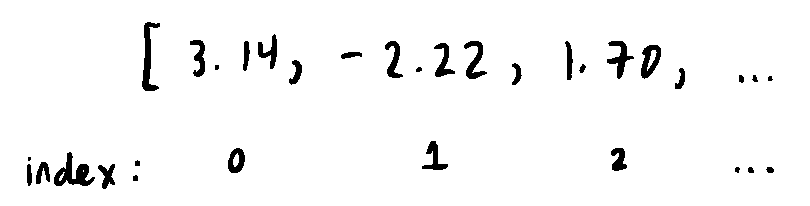
\includegraphics[width=\linewidth]{figs/array.pdf}
  \caption{A generic array, indexed from 0.} 
  \label{fig:array}
\end{figure}

From now on, we will try to think about data storage from the programming
side. From the programming side of things, it is often efficient and intuitive
to organize data such that lots of related information is kept close together.
The most common way to do this is an {\it array}\index{array}, which is
basically an ordered tuple\footnote{In Python, basic arrays are implemented as
lists.}. The $0\nth$ element of an array corresponds to that array's memory
address, and the addresses of all other data stored in that array are measured
relative to the address of this $0\nth$ element. Each element of an array is
labelled with an {\it index}, and one uses index $i$ to access array element
$i$. This is shown schematically in \figref{fig:array}.


The fundamental object we need to store is an $\SU(3)$ gauge field.
From \secref{sec:fields}, recall that this means we must associate four matrices
to each space-time point (because we live in four dimensions). Moreover each
matrix can be represented in a computer as an array; hence the overall
strategy is to create an ``array of subarrays".

Let us begin by storing a matrix in an array. This is relatively
straightforward. An $\SU(3)$ matrix is a $3\times3$ matrix with complex entries,
so a generic matrix $U_\mu(\fvec{x})\in\SU(3)$ at space-time site $\fvec{x}$
pointing in the $\muh$-direction can be represented with 18 real numbers as
\begin{equation}
U_\mu(\fvec{x})=\left(\begin{array}{ccc}
x_{00} + iy_{00} & x_{01} + iy_{01} & x_{02} + iy_{02} \\
x_{10} + iy_{10} & x_{11} + iy_{11} & x_{12} + iy_{12} \\
x_{20} + iy_{20} & x_{21} + iy_{21} & x_{22} + iy_{22} 
\end{array}\right),
\end{equation}
where each $x_{ij},y_{ij}\in\R$. This can be straightforwardly converted to an
18-component array of the form
\begin{equation}
[x_{00},~y_{00},~x_{01},~y_{01},~...,~x_{22},~y_{22}],
\end{equation}
and in practice this is exactly how we store each matrix as an array.

\begin{figure}
  \centering
  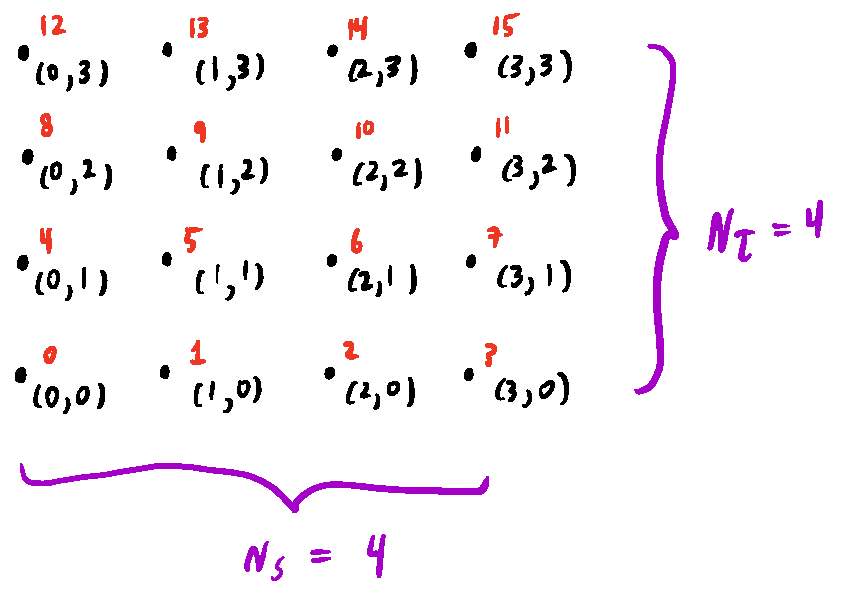
\includegraphics[width=\linewidth]{figs/indexing.pdf}
  \caption{How the sites of a lattice are indexed. In the above example, we
consider a 2-$d$ lattice with spatial extension $N_s=4$ and time extension
$N_\tau=4$. Each site is represented by a black dot and its 2-$d$ coordinate is
listed next to it. The site index is given in red.}
  \label{fig:index}
\end{figure}

Next we will need a way to assign an integer to a space-time coordinate. This is 
called {\it indexing}, and the way indexing goes is shown in \figref{fig:index},
which is a 2-$d$ example. By eye we can see the indexing pattern: we start with
sites at the ``bottom" of the lattice (at $t=0$), then increase our index as we
proceed from left to right (increasing $x$ from 0 to $N_s$). 
In 2-$d$, you can easily verify that the formula that accomplishes this is
\begin{equation}\label{eq:lex2d}
  \text{index}=x+yN_s.
\end{equation}
In four dimensions, this can be generalized to
\begin{equation}\label{eq:lex4d}
  \text{index}=x+yN_s+zN_s^2+tN_s^3.
\end{equation}
This indexing method is called {\it lexicographic
ordering}\index{lexicographic}. 

We are now ready to construct our array of subarrays. Let us call the array
containing the subarrays the ``superarray"\footnote{This is not common
terminology; I'm just trying to be pedagogical. Usually we simply refer to the
``superarray" as the ``gauge field".}. In our case, each subarray contains
the elements of a single link, which again is an $\SU(3)$ matrix.
We will organize our superarray such that all links pointing in the
$\hat{x}$-direction come first, followed by all the $\hat{y}$-links, then the
$\hat{z}$-links, then the $\hat{t}$-links\footnote{In principle there is no 
single ``correct" way to organize the links inside the
superarray; indeed the optimal ordering depends on details of the code. In many
code bases, when accessing links, one loops over the space-time directions. In
that case, having all data corresponding to a particular direction ``close
together" in memory saves a lot of computational effort, because the code has to
spend less time looking up links.}. Schematically, our superarray then looks
like
\begin{equation}
  \text{superarray}=\left[\{U_x\},~\{U_y\},~\{U_z\},~\{U_t\}\right],
\end{equation}
where $\{U_x\}$ indicates the set of all links pointing in the
$\hat{x}$-direction, and similarly for the other sets.
Each set $\{U_x\}$ then stores links $U_x(\fvec{x})$ in this order: according to
\equatref{eq:lex4d}, the link with index 0 comes first, followed by 1, and so
on. Hence this set is ordered like
\begin{equation}
\{U_x\} = \{ U_x(0),~U_x(1),~...,~U_x(N_s^3N_t-1)\},
\end{equation}
where now the argument of each $U$ is its lexicograhic index rather than its
space-time coordinate. This specifies completely how to store an $\SU(3)$ gauge
field in a large array.

To wrap up, let's figure out how large this array must be. Recall that each
$\SU(3)$ matrix in our implementation is represented by 18 real numbers.
If a real number is stored as a double-precision number, that number requires 8
bytes of memory. The total memory requirement for one $\SU(3)$ gauge field is then
\begin{equation}
\text{size}=\text{size of real}\times\text{number of dimensions}
             \times\text{ number of sites.}
\end{equation}
In four dimensions, the number of sites is $N_s^3N_t$, and so 
\begin{equation}\label{eq:latsize}
\text{size}=32N_s^3N_t\text{ bytes.}
\end{equation}

\section{Further studying}

If you have decided you
find lattice calculations interesting, so much so that you think you want to
pursue lattice research in grad school, I would recommend the following books on
the subject:
\begin{itemize}
\item {\it Quantum Chromodynamics on the Lattice: An Introductory Presentation}
by Gattringer and Lang~\cite{gattringer_quantum_2010} is probably the most pedagogical 
introduction to lattice calculations.
\item {\it Quantum Fields on a Lattice} by Montvay and 
M\"unster~\cite{montvay_quantum_1994} is a bit more
rigorous than Gattringer and Lang and contains a few other topics, like the
Higgs phase diagram. It is less pedagogical.
\item {\it Lattice Methods for Quantum Chromodynamics} by DeGrand and 
DeTar~\cite{degrand_lattice_2006} is
an excellent resource for a beginner and contains some extra information about
Symanzik improvement and lattice algorithms.
\end{itemize}
Some other books include Rothe's {\it Lattice Gauge Theories: An 
Introduction}~\cite{rothe_lattice_2005} and Smit's {\it Introduction to Quantum 
Fields on a Lattice}~\cite{smit_introduction_2002}. A book that rather
nicely connects LFT to {\it heavy-ion} experiments\index{heavy-ion experiment},
where we collide heavy nuclei like gold together in order to learn something
about strong interactions experimentally, can be found
in {\it The Deconfinement Transition of QCD: Theory Meets Experiment}
\cite{ratti_deconfinement_2021}. It will probably
be useful to you to at least have digital copies of all of them. In my
experience, when learning an extremely esoteric subject, it helps to have as
many references as possible so that you can see things explained in multiple
different ways.

Lattice calculations lie at the intersection of many disciplines in math,
physics, and scientific computing. Therefore if you want to get a deeper
understanding of the field, you should at least take courses that teach
\begin{itemize}
  \item calculus of more than one variable;
  \item linear algebra;
  \item differential equations;
  \item complex analysis;
  \item probability and statistics;
  \item numerical methods;
  \item special relativity;
  \item thermodynamics;
  \item statistical mechanics;
  \item electrodynamics;
  \item quantum mechanics; and
  \item quantum field theory.
\end{itemize}
If you have time, you can get an even deeper understanding of some niche topics
in the field if you also take courses that cover
\begin{itemize}
  \item topology;
  \item differential geometry;
  \item Lie groups;
  \item clean coding and object-oriented programming;
  \item accelerated computing;
  \item machine learning;
  \item phase transitions and critical phenomena;
  \item general relativity; and
  \item topical courses in contemporary particle physics.
\end{itemize}

I hope that you do choose to become a lattice practitioner. It's a big field
with lots of valuable knowledge, lots of ways to contribute depending on your
skills and interests, and the potential to have some role helping advance modern
particle physics. Thanks for reading these notes. I hope they were helpful to
you in some way.\\[5mm]
-David

\section*{Exercises}
\begin{enumerate}
  \item Looking at \equatref{eq:lex2d} and \eqref{eq:lex4d}, what do you think
should be the lexicographic indexing formula in 3-$d$? Draw a $4\times4\times4$
cube and verify that your formula works.
  \item The Fermilab-MILC-HPQCD collaboration generates some sizeable lattices.
One set of lattices has $N_s=144$ and $N_\tau=288$. Assuming the $\SU(3)$ gauge
field of this configuration is stored in
double precision, how many bytes are required? What about single precision?
\end{enumerate}

\bibliographystyle{unsrtnat}
\bibliography{bibliography}
